\documentclass{article}
\usepackage{pgf-pie}  % For creating pie charts
\usepackage{animate}  % For creating the animation

\begin{document}

\begin{figure}[h!]
    \centering
    \begin{animateinline}[autoplay, loop, controls]{1}  % 1 frame per second, autoplay, loop
        % Frame 1: Only first slice
        \frame{
            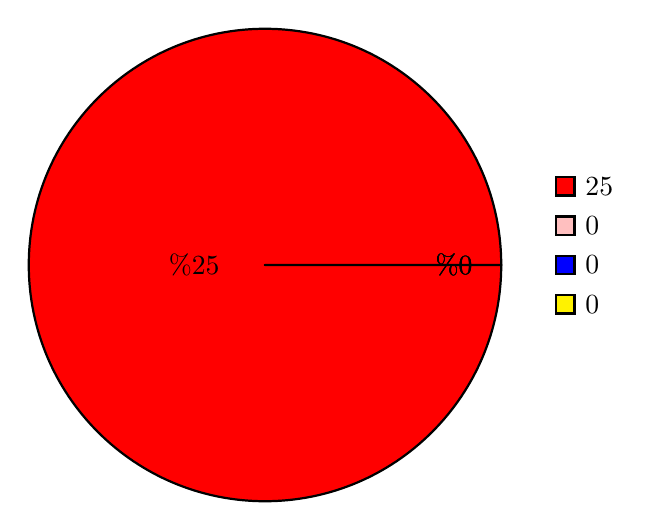
\begin{tikzpicture}
                \pie[sum=auto, text=legend, radius=3, before number=\%, color={red, pink, blue, yellow}]{
                    25, 0, 0, 0   % Only the first slice (25%) is drawn in this frame
                }
            \end{tikzpicture}
        }
        % Empty Frame: Introduce a 1-second delay before the next frame
        \frame{}
        
        % Frame 2: First slice + second slice
        \frame{
            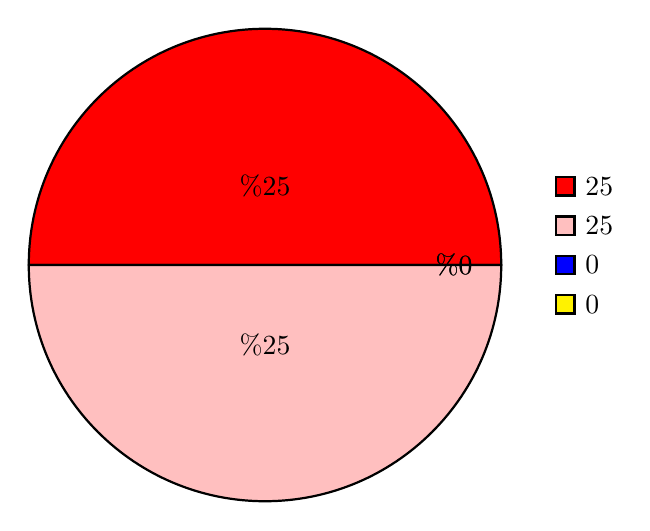
\begin{tikzpicture}
                \pie[sum=auto, text=legend, radius=3, before number=\%, color={red, pink, blue, yellow}]{
                    25, 25, 0, 0  % First two slices (25% each) are drawn
                }
            \end{tikzpicture}
        }
        % Empty Frame: Introduce a 1-second delay before the next frame
        \frame{}
        
        % Frame 3: First three slices
        \frame{
            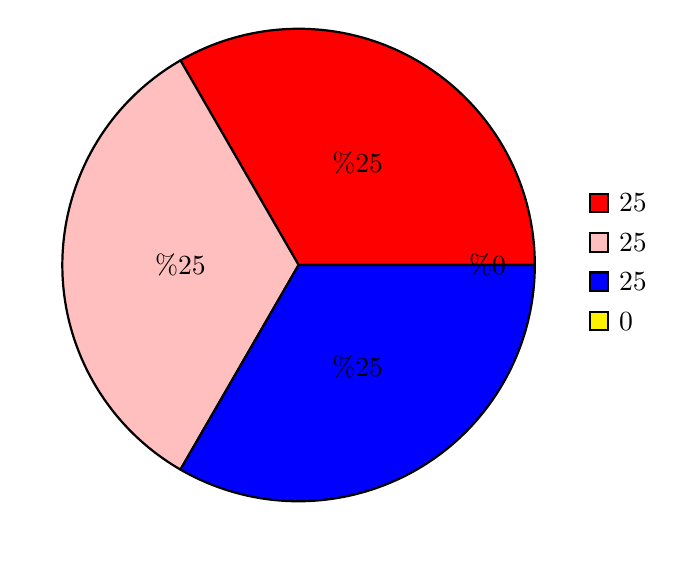
\begin{tikzpicture}
                \pie[sum=auto, text=legend, radius=3, before number=\%, color={red, pink, blue, yellow}]{
                    25, 25, 25, 0  % First three slices (25% each) are drawn
                }
            \end{tikzpicture}
        }
        % Empty Frame: Introduce a 1-second delay before the next frame
        \frame{}
        
        % Frame 4: All slices (complete pie)
        \frame{
            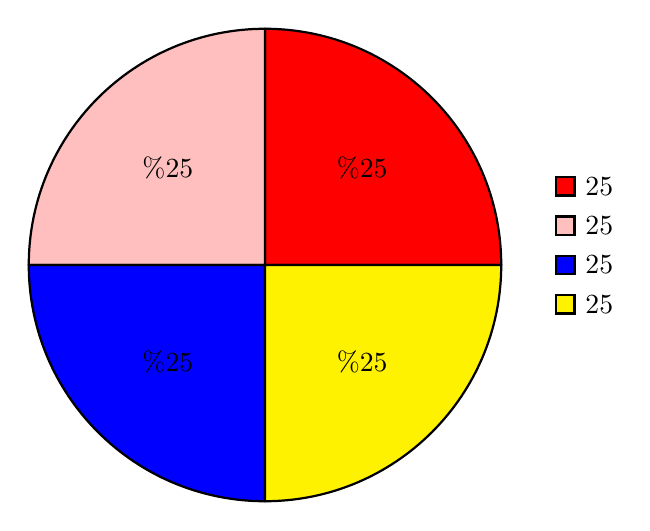
\begin{tikzpicture}
                \pie[sum=auto, text=legend, radius=3, before number=\%, color={red, pink, blue, yellow}]{
                    25, 25, 25, 25  % All four slices (25% each) are drawn
                }
            \end{tikzpicture}
        }
    \end{animateinline}
\end{figure}

\end{document}




